%%%%%%%%%%%%%%%%%%%%%%%%%%%%%%%%%%%%%%%%%%%%%%%%%%%%%%%%%%%%%%%%%%%%%%%%%%%%%%%%
% ICPP 2026 submission template (ACM acmart, sigconf, double-anonymous review).
% Per the ICPP 2026 CFP: "Please use the ACM format ... we recommend using
% \documentclass[sigconf,review,anonymous]{acmart} configuration for
% submissions prepared in LaTeX. Changes to the template (e.g., margin,
% font size) could lead to automatic rejection."
%%%%%%%%%%%%%%%%%%%%%%%%%%%%%%%%%%%%%%%%%%%%%%%%%%%%%%%%%%%%%%%%%%%%%%%%%%%%%%%%
\documentclass[sigconf,review,anonymous]{acmart}

% acmart already loads: amsmath, amssymb, amsfonts, graphicx, hyperref, xcolor.
% Only load what acmart does not provide.
\usepackage{tikz}
\usepackage{enumitem}
\usepackage{subcaption}
\usepackage{algorithm}
\usepackage{algpseudocode}

% Suppress ACM reference format / copyright box for the anonymous review PDF.
\settopmatter{printacmref=false}
\setcopyright{none}
\renewcommand\footnotetextcopyrightpermission[1]{}
\pagestyle{plain}

%-------------------------------------------------------------------------------
% Project-specific macros
%-------------------------------------------------------------------------------
\newcommand{\systemname}{DynaMoE}
\newcommand{\niparagraph}[1]{\smallskip\noindent\textbf{#1}}

% autoref name overrides
\renewcommand{\sectionautorefname}{\S}
\renewcommand{\subsectionautorefname}{\S}
\renewcommand{\subsubsectionautorefname}{\S}
\renewcommand{\figureautorefname}{Fig.}
\renewcommand{\equationautorefname}{Eq.}

%-------------------------------------------------------------------------------
% Front matter
%-------------------------------------------------------------------------------
\title{\systemname: Runtime Prefetch Horizon Control for Memory-Constrained Mixture-of-Experts Serving}

% Double-anonymous review: do not reveal author identity. The `anonymous`
% class option strips author/affiliation info from the rendered PDF, but
% acmart still requires the macros to be present.
\author{Anonymous Author(s)}
\affiliation{%
  \institution{Submission \#XXX}
  \country{}
}
\email{anonymous@icpp2026.submission}

%-------------------------------------------------------------------------------
\begin{document}
%-------------------------------------------------------------------------------

\begin{abstract}
A central bottleneck in serving Mixture-of-Experts (MoE) models on
memory-constrained accelerators is the temporal mismatch between
computation progress and expert parameter availability.
Existing cross-layer prefetching systems hide this mismatch by
forecasting expert usage and prefetching a fixed number of MoE layers
ahead, but this fixed horizon~$S$ either leaves transfers exposed on
the critical path (when~$S$ is too small) or triggers cache pollution
and eviction cascades (when~$S$ is too large), and we show that no
single offline~$S$ dominates across hardware, batches, and intra-batch
token diversity.
To address this, we propose treating~$S$ as a \emph{runtime control
variable} rather than a configuration knob, picking a different~$S_t$
at each control period in response to current stall and eviction
signals.
This reframing makes the prefetch depth track the per-period optimum,
recovering the wins of any fixed~$S$ on the configurations where it
would be best, simultaneously, and without offline tuning.
To realize this idea, we develop \systemname, a serving runtime whose
controller updates~$S$ via a bounded $\pm 1$ rule with hysteresis on
EMA-smoothed signals, at $O(1)$ per-update cost.
A CPU-side delta-adjusted random-forest forecaster supplies
confidence-weighted expert predictions without consuming GPU cycles.
A residency-aware two-tier expert cache and a cache-aware token router
bound the cost of misprediction so that every prediction error costs
at most one DMA, never a cascade of stalls.
We evaluate \systemname\ on three accelerators with very different
compute-to-bandwidth ratios (NVIDIA A6000, NVIDIA H20, Ascend 910B)
and three MoE models (DeepSeek-V2-Lite, Qwen1.5-MoE, Qwen2-MoE) under
a 20\,GB HBM cap.
Compared to a fixed-horizon proactive-prefetching baseline,
\systemname\ raises expert-activation prediction accuracy by an
average of $21.8\%$ (up to $30.4\%$) and reduces the cache-miss
latency component by a geometric mean of $\approx 13\times$ across
the eight supported model--device pairs (median $7\times$--$30\times$),
while never degrading configurations in which transfers are already
well overlapped.
\end{abstract}

\begin{CCSXML}
<ccs2012>
<concept>
<concept_id>10010520.10010575.10010755</concept_id>
<concept_desc>Computer systems organization~Heterogeneous (hybrid) systems</concept_desc>
<concept_significance>500</concept_significance>
</concept>
<concept>
<concept_id>10010147.10010257.10010321.10010333</concept_id>
<concept_desc>Computing methodologies~Massively parallel and high-performance simulations</concept_desc>
<concept_significance>300</concept_significance>
</concept>
<concept>
<concept_id>10010147.10010178.10010179.10010181</concept_id>
<concept_desc>Computing methodologies~Neural networks</concept_desc>
<concept_significance>300</concept_significance>
</concept>
</ccs2012>
\end{CCSXML}

\ccsdesc[500]{Computer systems organization~Heterogeneous (hybrid) systems}
\ccsdesc[300]{Computing methodologies~Massively parallel and high-performance simulations}
\ccsdesc[300]{Computing methodologies~Neural networks}

\keywords{Mixture-of-Experts, LLM serving, expert prefetching, GPU memory management, adaptive control, parallel inference}

\maketitle

\section{Introduction}
\label{sec:intro}

Mixture-of-Experts (MoE) architectures~\cite{jiang2024mixtral,masoudnia2014mixture,wang2025hmoe} let large language models (LLMs) scale parameter capacity without proportionally scaling per-token compute by activating only a small subset of experts per token~\cite{shazeer2017outrageously}. Designs like Switch Transformer~\cite{fedus2022switch}, GShard~\cite{lepikhin2020gshard}, and DeepSeek-V2~\cite{deepseekai2024deepseekv2strongeconomicalefficient} have made this routine. In latency-sensitive serving, however, MoE inference exposes a distinct systems bottleneck: expert weights are large, sparsely accessed, and rarely fit fully on the device, so \emph{when} and \emph{which} experts to move are as critical as routing itself.

The dominant mitigation today is \emph{cross-layer prefetching}: while executing layer~$\ell$, the runtime forecasts the experts needed by the next~$S$ MoE layers and overlaps their transfer with computation. ProMoE~\cite{song2024promoe}, ExpertFlow~\cite{he2024expertflow}, and Hobbit~\cite{tang2024hobbit} all instantiate this template; they choose the prefetch depth~$S$ \emph{offline} and reuse it across all requests. The depth itself, however, is what governs whether transfers ever land off the critical path. A too-small~$S$ leaves transfers unfinished when computation reaches layer~$\ell$, and the critical path accumulates \emph{exposed waiting latency}. A too-large~$S$ makes speculative residency exceed HBM capacity, evictions cascade, and \emph{cache pollution} amplifies subsequent miss latency. We measured this U-shaped tradeoff on three MoE models across three accelerators (\autoref{fig:M1}). At a fixed model and device, picking a sub-optimal~$S$ inflates end-to-end latency by up to $2.5\times$ as batch size changes and by up to $300\%$ as intra-batch token diversity changes (\autoref{sec:bg-motivation}). Existing fixed-horizon systems pay these inflations in full whenever the deployment differs from their tuning point.

The position of the U-shape minimum shifts with effective transfer bandwidth (a hardware property), with batch-induced contention (a workload property), and with intra-batch routing diversity (a per-request property). For any candidate offline~$S^*$, we can exhibit a workload on which some other~$S'\neq S^*$ is strictly better (\autoref{sec:bg-motivation}). Tuning~$S$ offline therefore amounts to picking the configuration on which to lose: the engineer chooses one device--workload pair on which to be optimal and accepts a multiplicative latency tax everywhere else. The right object is not a hyperparameter but a runtime control policy. A system that picks~$S_t$ at each control period in response to current stall and eviction signals can recover the wins of any fixed~$S$ \emph{simultaneously}---on the configuration where it would be best, and without offline tuning---because the controller is free to choose a different~$S$ for every (device, batch, request, layer) tuple it encounters.

We present \systemname, a serving runtime that turns the prefetch horizon~$S$ into a first-class control variable. \systemname\ has three coordinated layers (\autoref{fig:overview}(d)). A closed-loop controller updates~$S$ via a bounded $\pm 1$ rule with hysteresis on EMA-smoothed stall and eviction signals at $O(1)$ per-update cost (\autoref{sec:design:controller}). A CPU-side delta-adjusted forecaster refines pregate logits with token-, layer-, and horizon-aware features using a random forest that never touches the GPU (\autoref{sec:design:forecaster}). A residency-aware two-tier expert cache with cache-aware token routing bounds the cost of misprediction so that every prediction error costs at most one DMA, never a cascading stall (\autoref{sec:design:memory}).

\begin{figure}
    \centering
    {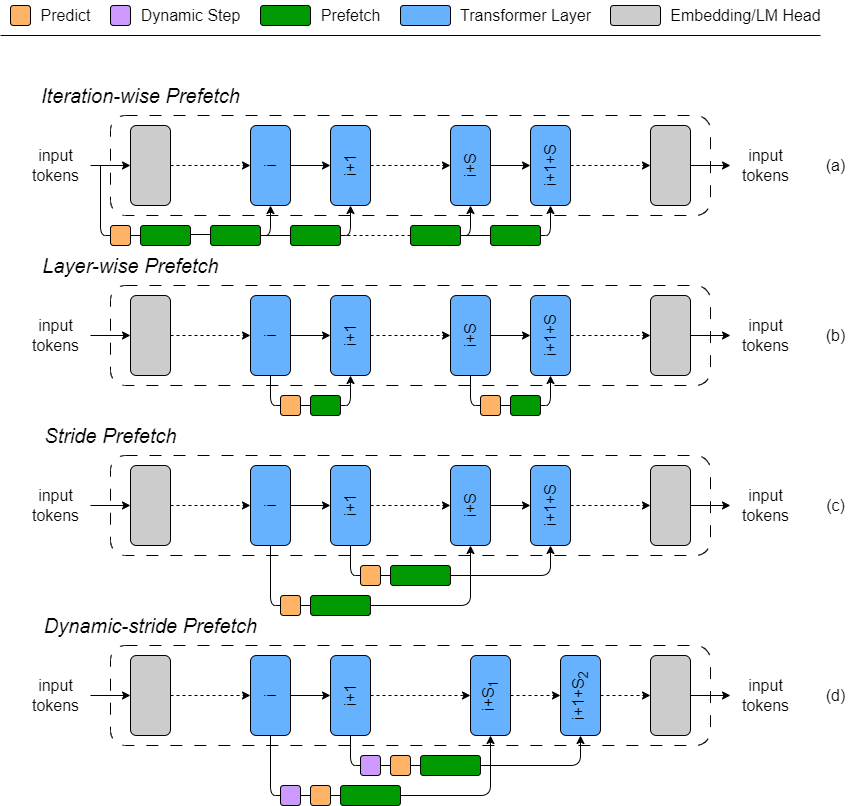
\includegraphics[width=0.99\linewidth]{figures/Candidate_prefetch_manners.png}}
    \vspace{-0.5em}
    \caption{Cross-layer expert prefetching strategies. (a)~Static
    expert--layer assignment, (b)~reactive routing, (c)~periodic
    prediction with a fixed horizon~$S$ (the template followed by
    ProMoE, ExpertFlow, and Hobbit), and (d)~\systemname's adaptive
    horizon control with feedback from runtime stall and eviction
    signals. (a)--(c) are dominated by some fixed~$S$ on every
    device--workload pair; (d) tracks the per-period optimum.}
    \label{fig:overview}
\end{figure}

We evaluate \systemname\ on NVIDIA A6000, NVIDIA H20, and Ascend 910B with DeepSeek-V2-Lite, Qwen1.5-MoE, and Qwen2-MoE under a 20\,GB HBM cap that forces expert swapping. Compared to a fixed-horizon proactive-prefetching baseline modeled after ProMoE~\cite{song2024promoe} and Eliseev~\emph{et al.}~\cite{eliseev2023fast}, \systemname\ raises expert-activation prediction accuracy by an average of $21.8\%$ (up to $30.4\%$) and reduces the cache-miss latency component by a geometric mean of $\approx 13\times$ across the eight supported model--device pairs (median $7\times$--$30\times$), while never degrading configurations in which the baseline already overlaps most transfers (e.g., Qwen2-MoE on H20). The controller's per-update cost stays under $50\,\mu$s on a commodity CPU.

We summarize our contributions as follows.
\begin{itemize}[leftmargin=1.4em, itemsep=2pt, topsep=2pt]
    \item We characterize the U-shaped overlap--pollution tradeoff of cross-layer prefetching on three MoE models and three accelerators, and show that for any candidate offline~$S^*$, the optimum lies elsewhere on some realistic workload---reframing~$S$ as a runtime control variable rather than a hyperparameter (\autoref{sec:bg-motivation}).
    \item We design a stable single-variable controller: a bounded $\pm 1$ update with hysteresis on EMA-smoothed signals tracks the per-period optimum at $O(1)$ per-update cost and is non-oscillatory by construction inside a configurable hysteresis band (\autoref{sec:design:controller}, Algorithm~\ref{alg:controller}).
    \item We co-design the forecaster and memory layer so that prediction errors are absorbed locally: a CPU-side delta-adjusted forecaster, a two-tier residency-aware cache, and cache-aware token routing together turn every prediction error into at most one DMA. We isolate the contribution of each layer via ablations on three accelerators (\autoref{sec:evaluation}).
\end{itemize}

\section{Background and Motivation}
\label{sec:bg-motivation}

\subsection{MoE Serving and Cross-Layer Prefetching}

\noindent
A Mixture-of-Experts (MoE) layer routes each token through only a small subset of its expert sub-networks~\cite{shazeer2017outrageously, fedus2021switch, yang2024xmoe, chen2022towards, zhou2022mixture}. At inference time, this sparsity reshapes the per-layer cost from being \emph{compute-bound} to being \emph{memory-bound}: per-token FLOPs drop with the activation ratio, but each MoE layer must fetch a different subset of expert weights, and an MoE model's expert footprint typically exceeds the device HBM by an order of magnitude. A serving runtime therefore cannot keep all experts resident; it must \emph{predict} which experts will be activated next and \emph{move} them onto the device ahead of execution.

\smallskip
\noindent
Cross-layer prefetching is the dominant template for hiding these expert transfers. While computing layer~$\ell$, the runtime forecasts the experts likely to be activated in the next~$S$ MoE layers and issues their transfers on a separate stream so that they overlap with the compute of layers~$\ell, \ldots, \ell{+}S{-}1$. We call~$S$ the \emph{prefetch horizon}. ProMoE~\cite{song2024promoe}, ExpertFlow~\cite{he2024expertflow}, and Hobbit~\cite{tang2024hobbit} all instantiate this template; they choose a single value of~$S$ at deployment time and reuse it across all requests. Crucially, $S$ does not change the model's routing semantics---it controls only how far ahead the system speculates.

\smallskip
\noindent
The choice of~$S$ is what determines whether expert transfers stay off the critical path. \autoref{fig:M1} plots latency against~$S$ for three MoE models on NVIDIA A6000 under a 20\,GB HBM cap. Each curve is U-shaped: below the U-minimum, transfers do not finish within the available compute window and the critical path accumulates exposed waiting; above it, speculative residency exceeds HBM capacity, evictions cascade, and cache pollution amplifies subsequent miss latency. The U-minimum sits at a different~$S$ for each model on the same device. Two questions follow: where does the U-minimum sit on a given deployment, and is it stable enough that we can find it offline?

\begin{figure}
    \centering
    {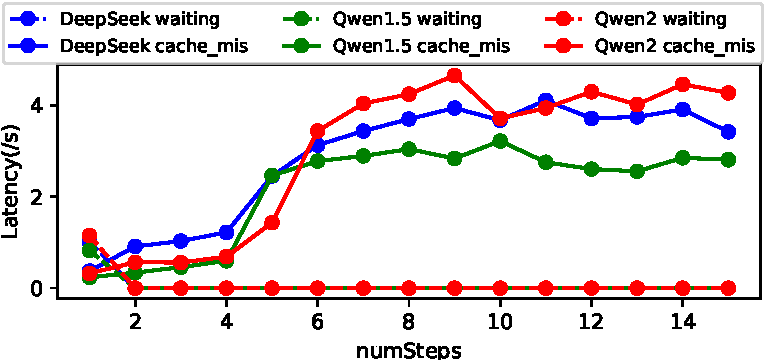
\includegraphics[width=0.99\linewidth]{figures/M1_numstep_latency.pdf}}
    \vspace{-0.5em}
    \caption{Latency vs.\ prefetch horizon~$S$ for three MoE models on
    NVIDIA A6000 under a 20\,GB HBM cap. The y-axis is waiting +
    cache-miss latency (s/request); the x-axis is~$S$ (number of MoE
    layers prefetched ahead). Each curve is U-shaped, and the
    U-minimum sits at a different~$S$ for each model. We show in
    \autoref{sec:bg-motivation:variance} that the minimum also moves
    across devices, batches, and intra-batch token compositions, so
    no offline-tuned~$S$ is robust.}
    \label{fig:M1}
\end{figure}

\subsection{The Optimum Moves Along Three Independent Axes}
\label{sec:bg-motivation:variance}

\noindent
The U-minimum is not stable. Three factors, each independent of the others, shift it. We discuss each in turn and connect it to the failure mode of fixed-horizon systems.

\paragraph{Hardware bandwidth.}
The accelerators used in this work span an order of magnitude in effective host--device bandwidth, from $\sim 8$\,GB/s on AMD RX~6500XT to $\sim 128$\,GB/s on NVIDIA H20 and Ascend~910B. The transfer time of a layer's experts scales inversely with this bandwidth, while the per-layer compute time scales with FLOPs throughput; their ratio determines how many compute-layers' worth of overlap window is available to hide one layer's transfer. On a fast interconnect a small~$S$ already fits transfers inside the overlap window; on a slow one a much larger~$S$ is needed. A fixed-horizon system tuned for one accelerator therefore exposes systematic stalls when migrated to a slower interconnect or a co-tenanted GPU where effective bandwidth has dropped---this is precisely the cross-device brittleness of ProMoE-style runtimes.

\paragraph{Batch scale.}
Even on fixed hardware, the optimal~$S$ shifts with batch size. Larger batches amortize per-layer overhead but also widen the set of concurrently demanded experts and shrink each expert's per-token overlap budget. To make this concrete, let $E_{\text{req}}$ be the experts requested by a batch over the next~$S$ layers, $\hat{E}$ the experts actually prefetched, and $E_{\text{hit}} = E_{\text{req}} \cap \hat{E}$ those that arrive before they are needed. The expert miss ratio is
$
R_{\text{miss}} = 1 - \tfrac{|E_{\text{hit}}|}{|E_{\text{req}}|}.
$
As batch-induced demand diversity grows, $|E_{\text{req}}|$ grows faster than $S$ can keep up, so $R_{\text{miss}}$ rises. \autoref{fig:M3} shows that holding~$S$ fixed and sweeping batch size from 1 to 32 inflates the waiting component of latency by up to $2.5\times$ while the cache-miss component can simultaneously decrease as residency stabilizes. The two components move in opposite directions, so no single~$S$ minimizes both---a fixed-horizon system is forced to trade one for the other.

\begin{figure}
    \centering
    {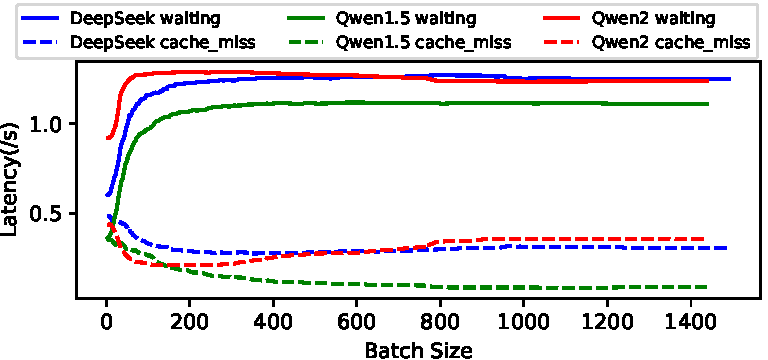
\includegraphics[width=0.99\linewidth]{figures/M3_batchsize_latency.pdf}}
    \vspace{-0.5em}
    \caption{Latency components vs.\ batch size at a fixed~$S$ on
    A6000. The waiting component grows non-monotonically with batch
    size (more concurrent requests $\Rightarrow$ more concurrently
    demanded experts $\Rightarrow$ less per-expert overlap window),
    increasing by up to $2.5\times$, while the cache-miss component
    can decrease as residency stabilizes. The two components move in
    opposite directions, which is precisely why a single offline~$S$
    cannot be optimal across batch sizes.}
    \label{fig:M3}
\end{figure}

\paragraph{Intra-batch token diversity.}
At fixed batch size, requests with different token compositions activate different sets of experts in subsequent layers. We use a lightweight proxy for intra-batch diversity, the sum of pairwise embedding distances:
\[
\text{Dist}(\mathbf{t}) = \sum_{1 \le i < j \le k} \lVert \mathbf{v}_{t_i} - \mathbf{v}_{t_j} \rVert_2,
\]
where $\mathbf{v}_{t_i}$ is the embedding of token $t_i$. \autoref{fig:M5} plots the number of distinct experts activated per layer against batch size and $\text{Dist}(\mathbf{t})$ on three MoE models. At a fixed batch size, requests with high semantic dispersion activate noticeably more experts and exhibit up to $300\%$ end-to-end latency variation compared to low-dispersion requests with the same batch size. A fixed-horizon system that chooses~$S$ on a representative low-dispersion batch therefore systematically under-prefetches on diverse batches, even when the deployment hardware and batch size are unchanged.

\begin{figure}
    \centering
    {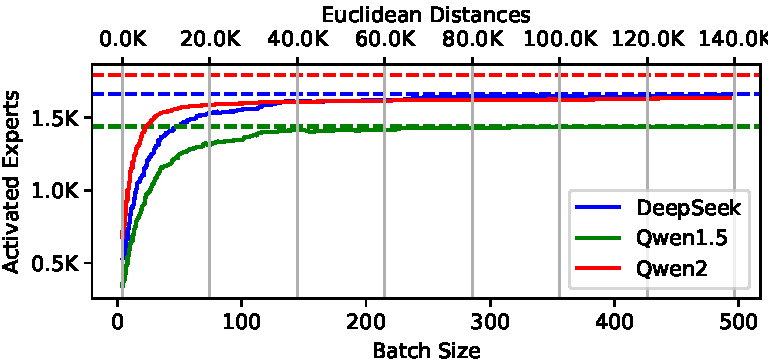
\includegraphics[width=0.99\linewidth]{figures/M5_DeepSeek_Qwen1.5_Qwen2.pdf}}
    \vspace{-0.5em}
    \caption{Number of distinct experts activated per layer vs.\
    batch size (x-axis) and the embedding-dispersion proxy
    $\mathrm{Dist}(\mathbf{t})$ (color), for DeepSeek-V2-Lite,
    Qwen1.5-MoE, and Qwen2-MoE. At fixed batch size, high-dispersion
    requests activate noticeably more experts and incur up to
    $300\%$ latency variation, so dispersion is a useful
    per-request signal for the controller, on top of batch size.}
    \label{fig:M5}
\end{figure}

\subsection{Implications for System Design}
\label{sec:bg-motivation:implications}

\noindent
Putting the three axes together, the U-minimum drifts continuously across (device, workload, request) tuples. For any candidate offline~$S^*$, we can construct a deployment in which some other~$S' \neq S^*$ is strictly better, and we exhibit such cases in our evaluation (\autoref{sec:evaluation}). Tuning~$S$ offline therefore amounts to picking the configuration on which to lose: the engineer chooses one device--workload pair to optimize and accepts a multiplicative latency tax everywhere else. The right object is not a hyperparameter but a control policy that chooses~$S_t$ at each control period in response to current runtime signals. Building such a policy means solving three coupled sub-problems---deriving a stable~$S_t$ from partial, noisy observations of bandwidth, demand, and cache state; predicting which experts will be needed over the next~$S_t$ layers without competing for GPU cycles; and bounding the cost of misprediction so that errors cause at most one DMA, never a cascade of stalls---which we address in \autoref{sec:design:controller}, \autoref{sec:design:forecaster}, and \autoref{sec:design:memory}, respectively.

\section{System Design}
\label{sec:design}

\noindent
This section answers the three coupled sub-problems raised in
\autoref{sec:bg-motivation:implications}, layer by layer:
\autoref{sec:design:controller} derives a stable~$S_t$ from partial
observations; \autoref{sec:design:forecaster} predicts the experts
needed over the next~$S_t$ layers without consuming GPU cycles; and
\autoref{sec:design:memory} bounds the cost of misprediction so that
errors cause at most one DMA, never a cascade of stalls. We start
with the system overview that ties them together
(\autoref{sec:design:overview}).

\subsection{Overview and Architecture}
\label{sec:design:overview}

\systemname\ converts MoE inference into a closed-loop scheduling
problem over a single scalar~$S_t$. The system has three layers
(\autoref{fig:architecture}). The \emph{controller}
(\autoref{sec:design:controller}) updates~$S_t$ from EMA-smoothed
runtime signals at constant per-update cost. The \emph{forecaster}
(\autoref{sec:design:forecaster}) predicts the experts likely to be
activated over the next~$S_t$ layers using token-, layer-, and
horizon-aware features, on the CPU. The \emph{memory layer}
(\autoref{sec:design:memory}) materializes the forecast through
asynchronous transfers, a two-tier cache that protects high-reuse
experts, and cache-aware token routing that lets cache misses be
absorbed in parallel with resident-expert execution.

\begin{figure}
    \centering
    {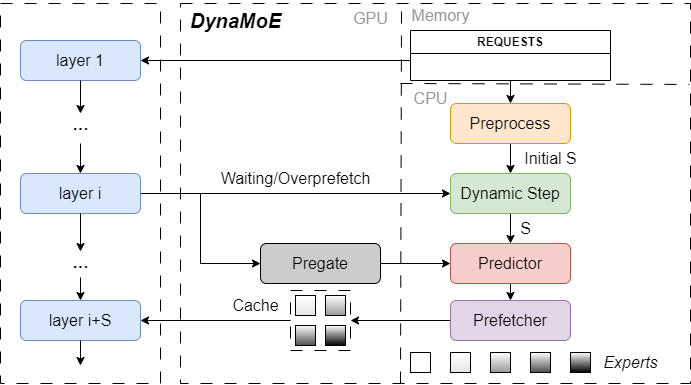
\includegraphics[width=0.99\linewidth]{figures/architecture.png}}
    \vspace{-0.5em}
    \caption{Architecture of \systemname.
    \emph{Online path:}
    (1)~per-layer hooks read smoothed waiting and miss signals
    $(\tilde{w}_t,\tilde{m}_t)$;
    (2)~the controller updates the horizon~$S_t$
    (\autoref{alg:controller});
    (3)~the forecaster emits the expert set $\hat{E}_{\ell+1..\ell+S_t}$
    and a confidence score;
    (4)~the two-tier cache issues asynchronous prefetches for
    non-resident experts on a dedicated transfer stream;
    (5)~the cache-aware router executes tokens whose experts are
    already resident first, deferring the rest until prefetch
    completes.
    \emph{Offline path:} the forecaster's CPU-side random forest is
    trained from logged $(\mathbf{t},\ell,S,\mathbf{a})$ tuples; no GPU
    cycles are spent on prediction at serving time.}
    \label{fig:architecture}
\end{figure}

Each control period~$T_u$, the controller solves the following
optimization:
\begin{equation}
\label{eq:formulation}
\begin{aligned}
\min_{S_{t+1}\in\mathbb{Z}\cap[S_{\min},S_{\max}]} \;
   & \tilde{L}_{\text{wait}}(S_{t+1}) + \lambda\,\tilde{L}_{\text{miss}}(S_{t+1}), \\[-1pt]
\text{s.t.}\quad
   & \text{(C1)}\;\mathrm{occ}(\hat{E}_{\ell+1..\ell+S_{t+1}})\le M_{\text{HBM}}, \\[-1pt]
   & \text{(C2)}\;|S_{t+1}-S_t|\le 1, \\[-1pt]
   & \text{(C3)}\;\text{prefetch}\subseteq\hat{E}_{\ell+1..\ell+S_{t+1}}.
\end{aligned}
\end{equation}
$\tilde{L}_{\text{wait}}$ and $\tilde{L}_{\text{miss}}$ are
EMA-smoothed exposed-stall and eviction-pressure proxies
(\autoref{sec:design:controller}); $\hat{E}$ is the forecaster's
prediction (\autoref{sec:design:forecaster}); $M_{\text{HBM}}$ is the
expert residency budget. (C1) keeps each candidate~$S$ realizable
under the HBM cap, (C2) bounds per-step change so the controller
cannot oscillate, and (C3) keeps speculative prefetching restricted
to the current prediction set. \systemname\ exposes only two scalar
hyperparameters---the regime weight~$\lambda$ and the hysteresis
threshold~$\theta_h$ used by the controller---both fixed once at
startup.

The rest of this section answers, in order:
\begin{itemize}[leftmargin=1.4em, itemsep=2pt, topsep=2pt]
    \item \textbf{Q1.}\,How can the controller pick a stable~$S_t$ from
    partial, noisy observations of bandwidth, demand, and cache state?
    (\autoref{sec:design:controller})
    \item \textbf{Q2.}\,How can a predictor extend pregate signals over
    long horizons without competing for GPU cycles?
    (\autoref{sec:design:forecaster})
    \item \textbf{Q3.}\,How can the memory layer bound the cost of
    misprediction so that errors cause at most one DMA, never a
    cascade of stalls? (\autoref{sec:design:memory})
\end{itemize}

\subsection{Adaptive Controller}
\label{sec:design:controller}

The controller maintains EMA-smoothed estimates of two runtime
signals: $\tilde{w}_t = \mathrm{EMA}_\alpha(w_t)$ for exposed waiting
(the fraction of MoE-layer time spent stalled on a missing expert)
and $\tilde{m}_t = \mathrm{EMA}_\alpha(m_t)$ for pollution pressure
(evictions per miss-induced refill). Smoothing decouples the
controller from per-layer noise without introducing learned state.
The signed quantity $\Delta_t = \tilde{w}_t - \lambda\,\tilde{m}_t$
identifies the dominant failure mode at each control period:
$\Delta_t > 0$ means waiting dominates (under-prefetch), $\Delta_t < 0$
means pollution dominates (over-prefetch); the weight $\lambda$ trades
off the two costs, and we use $\lambda = 1$ throughout this paper.

The controller updates~$S$ by at most one layer per period inside a
hysteresis band of width~$\theta_h$:
$S_{t+1} = \min(S_t{+}1, S_{\max})$ if $\Delta_t > \theta_h$;
$\max(S_t{-}1, S_{\min})$ if $\Delta_t < -\theta_h$; and $S_t$
otherwise. The rule satisfies constraint~(C2) of
\autoref{eq:formulation} by construction. A short informal argument
explains stability. Inside the band the rule is the identity, so once
the regime indicator enters the band, $S_t$ is fixed. Outside the
band, $|\Delta_t|>\theta_h$ deterministically pushes $S_t$ toward the
regime knee at one layer per period; bounded by
$[S_{\min}, S_{\max}]$, the trajectory reaches a band-boundary in at
most $S_{\max}-S_{\min}$ periods. EMA smoothing ($\alpha\in[0,1)$)
exponentially attenuates the indicator's response to any single noisy
observation, so the controller cannot be flipped in and out of the
band by a transient spike.

\autoref{alg:controller} summarizes one control period. The per-update
cost is $O(1)$; the aggregate per-request cost is
$O(L_{\text{MoE}})$, independent of model size, batch size, and~$S$.
An update completes in under $50\,\mu$s on a commodity CPU in our
implementation. Lines~1--2 update the smoothed signals; line~3
computes $\Delta_t$; lines~4--10 are the $\pm 1$ rule above. Across
one request the controller has three typical phases: in the first
periods after a workload change $\Delta_t$ is consistently outside
the band and~$S$ moves monotonically toward the new knee; around the
knee $\Delta_t$ enters the band and~$S$ holds; under sustained drift
(a co-tenant traffic spike, or a batch with very different
intra-batch dispersion) $\Delta_t$ leaves the band again and the
controller re-converges.

Before any feedback is available, $S$ is initialized from a coarse
analytical estimate using forecaster output and recent transfer
timing. With $N_e$ predicted experts per layer of size $E_s$ bytes,
measured effective bandwidth $C_s$, and per-layer compute time $T_l$,
the transfer of one layer's experts takes $N_e E_s / C_s$ seconds,
which the controller hides behind $S\cdot T_l$ seconds of compute.
Solving for $S$ gives
\(
S_0 = \lceil N_e E_s / (C_s T_l) \rceil,
\)
in units of MoE layers. The closed-loop rule then takes over at the
first control period; mis-set $S_0$ only delays convergence.

\begin{algorithm}[t]
\caption{\systemname\ adaptive horizon controller (per control period~$T_u$).}
\label{alg:controller}
\begin{algorithmic}[1]
\Require EMA factor $\alpha$, regime weight $\lambda$, hysteresis $\theta_h$, bounds $[S_{\min}, S_{\max}]$
\Require previous state $(\tilde{w}_{t-1}, \tilde{m}_{t-1}, S_t)$, raw counters $w_t, m_t$
\Ensure next horizon $S_{t+1}$
\State $\tilde{w}_t \gets \alpha\,\tilde{w}_{t-1} + (1-\alpha)\,w_t$ \Comment{smoothed waiting}
\State $\tilde{m}_t \gets \alpha\,\tilde{m}_{t-1} + (1-\alpha)\,m_t$ \Comment{smoothed pollution}
\State $\Delta_t \gets \tilde{w}_t - \lambda\,\tilde{m}_t$         \Comment{regime indicator}
\If{$\Delta_t > \theta_h$}                                         \Comment{stall-dominated}
    \State $S_{t+1} \gets \min(S_t + 1,\, S_{\max})$
\ElsIf{$\Delta_t < -\theta_h$}                                     \Comment{pollution-dominated}
    \State $S_{t+1} \gets \max(S_t - 1,\, S_{\min})$
\Else                                                              \Comment{within hysteresis band}
    \State $S_{t+1} \gets S_t$
\EndIf
\State \Return $S_{t+1}$
\end{algorithmic}
\end{algorithm}

\subsection{Forecasting Layer}
\label{sec:design:forecaster}

For each request \systemname\ logs a tuple
$(\mathbf{t}_i, \ell_i, \mathbf{p}_i, \mathbf{a}_i, s_i)$ per MoE
layer, recording token IDs, layer index, pregate-predicted experts,
actually activated experts, and the step size in effect. Tokens are
embedded through a frozen table $\mathbf{E}\in\mathbb{R}^{V\times d}$
and mean-pooled into a request descriptor
$\mathbf{e}=\tfrac{1}{k}\sum_{i=1}^k \mathbf{E}_{t_i}$; the per-layer
feature $\mathbf{x} = [\mathbf{e},\, S,\, \ell,\, \text{prev\_act}]$
concatenates this descriptor with the current horizon, layer index,
and a binary vector of prior-layer activations. A CPU-side random
forest regresses $\mathbf{x}$ to the multi-hot label $\mathbf{y}$ of
actually activated experts under MSE. We chose a forest over a deep
predictor for three system-level reasons: it adds no GPU interference,
its prediction latency at control-period granularity is sub-millisecond
on commodity CPUs and never blocks the inference critical path, and
its accuracy is stable across our model groups
(\autoref{sec:evaluation}).

Raw pregate outputs exhibit layer-local noise. The forecaster learns
the deviation $\Delta$ between pregate predictions and actual
activations and produces a refined prediction
$\hat{\mathbf{y}} = \mathbf{p} + \Delta$. When an identical
(token-sequence, layer, $S$) tuple reoccurs, the cached prediction is
reused; otherwise the system falls back to the model's own top-$k$
router logits, so \systemname\ never blocks waiting for prediction.
The forecaster passes two signals to the controller: the expected
number of experts per future layer~$N_e$ (used in $S_0$ in
\autoref{sec:design:controller}), and a confidence score derived from
historical prediction accuracy. Low confidence widens $\hat{E}$,
which tightens (C1) of \autoref{eq:formulation} and implicitly shrinks
$S$, so the controller becomes conservative when the predictor is
uncertain.

\begin{figure}[t]
    \centering
    {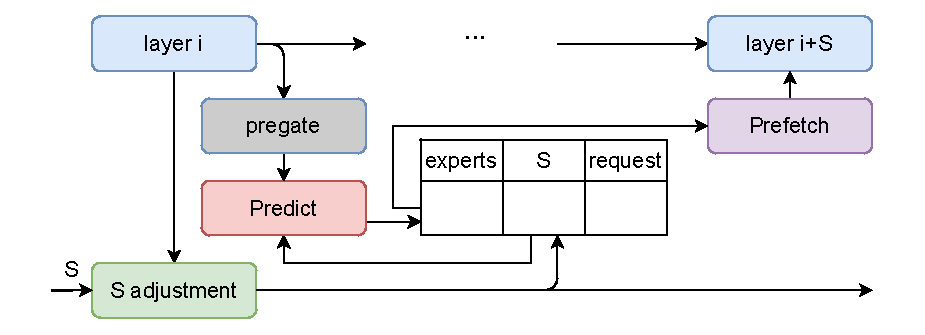
\includegraphics[width=0.99\linewidth]{figures/codesign.pdf}}
    \vspace{-0.5em}
    \caption{Co-design of the forecaster and the controller in
    \systemname. The forecaster provides $\hat{E}_{\ell+1..\ell+S}$
    and a confidence score; the controller consumes the predicted
    expert count $N_e$ to compute $S_0$ at startup, and the smoothed
    counters $\tilde{w}_t, \tilde{m}_t$ to update~$S$ at each period.
    Low-confidence forecasts widen $|\hat{E}|$, which tightens the
    HBM constraint~(C1) and implicitly shrinks~$S$, so the
    controller automatically becomes conservative when the predictor
    is uncertain.}
    \label{fig:codesign}
\end{figure}


\subsection{Expert Memory Management}
\label{sec:design:memory}

The memory layer translates forecasts into residency decisions and
returns cache statistics to the controller. It is designed so that a
mispredicted expert costs at most one extra DMA, never a cascading
stall, which is what lets the controller safely explore larger~$S$
without paying eviction--reload amplification.

\textbf{Two-tier LRU.}
Rather than a single eviction queue, \systemname\ maintains two LRU
structures: \texttt{LRU\_high} holds experts with demonstrated reuse
(recently accessed or imminently predicted), while \texttt{LRU\_low}
holds the rest. Evictions are drawn preferentially from
\texttt{LRU\_low}, which spills to host DRAM and preserves high-reuse
experts on the device. This two-tier design directly addresses a
pathology of single-tier LRU on layer-wise MoE: experts from the
first~$S$ layers are reused later during decoding, yet a single LRU
prematurely evicts them as more recent layers fill the queue.

\textbf{Prefetch--cache feedback loop.}
Memory management and the controller form a closed loop:
\textit{(1)} before computing~$S$, the controller queries current cache
occupancy to estimate effective bandwidth and the anticipated eviction
cost; \textit{(2)} after each prefetch completes, observed transfer
time updates the bandwidth estimate $C_s$ used in $S_0$
(\autoref{sec:design:controller}); \textit{(3)} cache hit/miss counters
feed $\tilde{m}_t$ in \autoref{alg:controller}. This feedback prevents
the runtime from issuing prefetches that would themselves trigger
evictions of experts the controller still expects to use.

\textbf{Cache-aware routing.}
A cache miss inside an MoE layer manifests as an asynchronous stall.
\systemname\ exploits the asynchrony by routing tokens to experts in
order of cache residency: tokens whose experts are already resident
execute first; tokens that would trigger a fault are deferred until
the corresponding swap-in completes, which happens in parallel with
the resident-expert path. Compared with conventional sequential
swap-in (where every miss blocks), this overlap reduces the exposed
component of cache-miss latency without altering routing semantics.
\section{Implementation}
\label{sec:implementation}

We implement \systemname\ as a drop-in runtime layer on top of HuggingFace
Transformers~\cite{wolf2020transformers}, with $\sim$4.5K lines of Python
and $\sim$0.6K lines of CUDA. The same Python codebase compiles for both
NVIDIA (PyTorch 2.3 / CUDA 12.2) and Ascend (CANN 7.0): a thin $\sim$150-LoC
device shim hides the difference between CUDA streams and the Ascend runtime
equivalents, so the controller and forecaster are device-independent. The
implementation modifies neither the model architecture nor the routing/gating
semantics, and can be swapped in front of any MoE model that follows
HuggingFace's \texttt{*MoeSparseMoeBlock} convention.

The forecaster is trained from $(\mathbf{t}, \ell, S, \mathbf{a})$ tuples
logged in a fixed-size pinned ring buffer (default 64K entries) during
serving. Retraining runs on the controller's CPU thread once per epoch
(10K requests or 60 seconds, whichever comes first) and never touches the
GPU. On a previously unseen model the buffer is empty for the first epoch
and the forecaster falls back to the model's own pregate top-$k$, so
\systemname\ degrades to a baseline-equivalent state at cold start rather
than failing.

\niparagraph{Latency attribution.}
For each MoE layer the runtime emits four \texttt{torch.cuda.Event}
timestamps---compute begin, compute end, first stall on a missing expert,
and stall release---and aggregates them in a per-request ring buffer. The
difference between stall release and stall begin is the \emph{exposed
waiting} component; the time spent inside the swap-in path is the
\emph{cache-miss} component; compute time is reported separately. The
breakdown plotted in \autoref{sec:evaluation}, including
Tables~\ref{tab:Dynamic_baseline}--\ref{tab:Dynamic_CCR}, is read directly
from these counters. Seeds are fixed for ShareGPT bucketing and forecaster
training; we will release the runtime, device shim, training pipeline, and
benchmark harness at the camera-ready URL.

\section{Evaluation}
\label{sec:evaluation}

We evaluate \systemname\ on three accelerators with very different
compute-to-bandwidth ratios and three MoE models under a 20\,GB HBM
cap. Throughout, we report two latency components measured by the
instrumentation in \autoref{sec:implementation}: \emph{exposed
waiting} (stall time not overlapped by compute) and \emph{cache-miss
latency} (time spent inside the swap-in path). Compute time is
reported separately and excluded from both. We summarize the headline
findings as follows:

\begin{itemize}[leftmargin=1.4em, itemsep=2pt, topsep=2pt]
    \item \systemname\ reduces the cache-miss latency component
    relative to a fixed-horizon baseline by a geometric mean of
    $\approx 13\times$ across the eight supported model--device pairs,
    while never degrading configurations in which the baseline
    already overlaps most transfers (\autoref{sec:eval:q1}).
    \item Each component contributes independently: the forecaster
    raises prediction accuracy by $21.8\%$ on average (up to
    $30.4\%$, \autoref{sec:eval:predictor}); the two-tier cache
    prevents the eviction--reload cliff that fixed-LRU suffers near
    $S\approx 4$ (\autoref{sec:eval:memory}); cache-aware routing
    suppresses the residual cache-miss component on H20, where
    higher compute throughput exposes more transfer time
    (\autoref{sec:eval:routing}).
    \item Aggregate runtime overhead is below $50\,\mu$s per
    controller update on a commodity CPU, and the forecaster's
    sub-millisecond inference never blocks the GPU critical path
    (\autoref{sec:eval:overhead}).
\end{itemize}

\subsection{Experiment Setup}

\niparagraph{Testbeds.}
All experiments were conducted on three accelerator platforms:
NVIDIA A6000~\cite{nvidiaA6000datasheet} (64~GB/s transfer bandwidth),
NVIDIA H20 (128~GB/s), and Ascend 910B (128~GB/s).
\systemname\ is implemented in Python and CUDA based on the Transformers
framework~\cite{wolf2020transformers}.
To reduce memory fragmentation and enable fine-grained expert residency control,
GPU HBM and host DRAM are managed in block granularity, with dynamic allocation
driven by runtime demand.
Expert swap-in/out transfers are issued on a dedicated CUDA stream to enable
overlap with compute, while a separate CPU thread tracks transfer progress and
memory block states.
We enable continuous batching to emulate serving-style throughput-oriented
execution.

\niparagraph{Workloads and Models.}
Requests are sampled from ShareGPT~\cite{ShareGPT_Vicuna_unfiltered}.
To mitigate heavy-tailed length distribution, we bucket requests by prompt length
and sample up to 50 requests per bucket (within $\pm 5\%$ length variation).
We evaluate three MoE models: DeepSeek-V2-Lite~\cite{DeepSeekCoderV2LiteBase, bi2024deepseek, deepseekai2024deepseekv2strongeconomicalefficient},
Qwen1.5~\cite{Qwen15MoEA27B, qwen_moe}, and Qwen2.0~\cite{Qwen257BA14BInstructGPTQInt4, qwen2}.
We apply INT4 quantization to Qwen2.0 where supported.

\niparagraph{Memory cap and comparability.}
To emulate resource-constrained serving, we cap GPU memory at 20~GB on all
platforms.
This cap forces expert residency competition and makes cache behavior observable.
Ascend 910B currently lacks INT4 support in our software stack, which prevents
running Qwen2.0 under the same 20~GB cap.
We therefore report Qwen2.0 results on A6000 and H20, and report DeepSeek/Qwen1.5
on all three devices.
This limitation is explicitly reflected in tables and does not affect our
cross-device conclusions about the mechanisms of \systemname, which are validated
on two MoE models across all platforms.

\niparagraph{Baselines.}
We compare \systemname\ against a baseline implementation built on Transformers
with representative proactive expert-loading components.
Specifically, the baseline incorporates (i) periodic cross-layer prediction in
the style of ProMoE~\cite{song2024promoe}, and (ii) pregate-based signals commonly
used to approximate upcoming expert activations~\cite{eliseev2023fast}.
We use the term \emph{Baseline} to denote this combined implementation.
When focusing on prediction accuracy alone, we separately report pregate accuracy
and compare against our Predictor (and discuss trend differences relative to
periodic prediction).

\subsection{Q1: Overall Waiting Latency Declines}
\label{sec:eval:q1}

We first evaluate the end-to-end impact of \systemname\ on exposed waiting and
cache-miss latency under memory-capped inference.
Conceptually, \systemname\ reduces waiting by (i) forecasting the experts that will
be needed before execution reaches them, (ii) prefetching these experts early enough
to overlap transfer with compute, and (iii) adapting the forecasting horizon (step
size) to match the current compute--communication ratio and workload dynamics.

\begin{figure*}
    \centering
    \begin{subfigure}{0.32\linewidth}
        \centering
        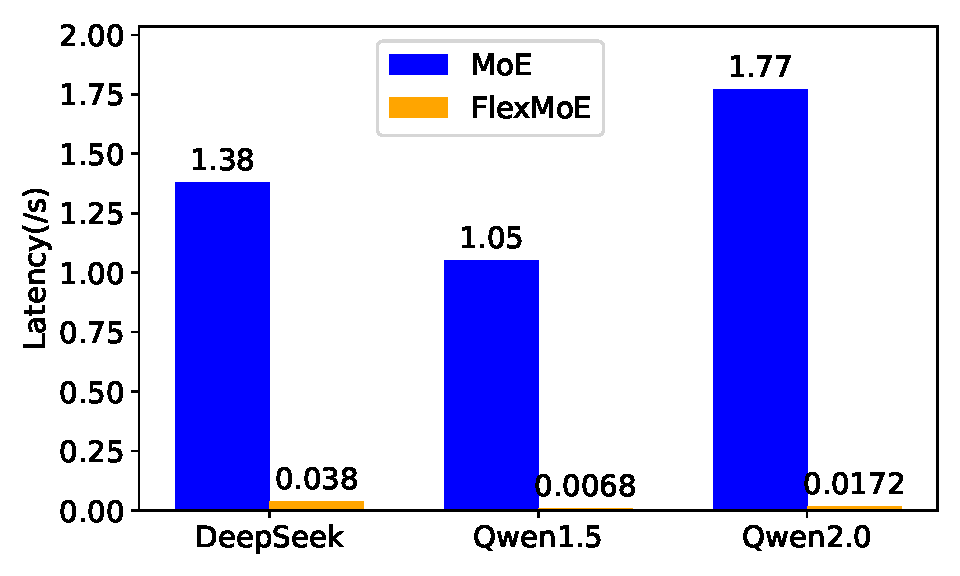
\includegraphics[width=0.99\linewidth]{figures/E2.pdf}
        \caption{NVIDIA A6000}
    \end{subfigure}
    \begin{subfigure}{0.32\linewidth}
        \centering
        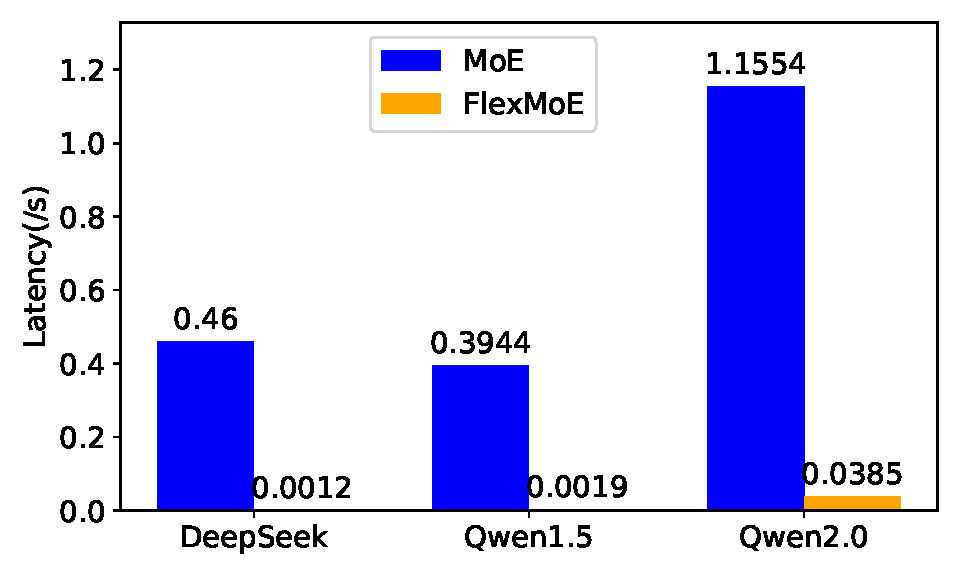
\includegraphics[width=0.99\linewidth]{figures/E2_H20.pdf}
        \caption{NVIDIA H20}
    \end{subfigure}
    \begin{subfigure}{0.32\linewidth}
        \centering
        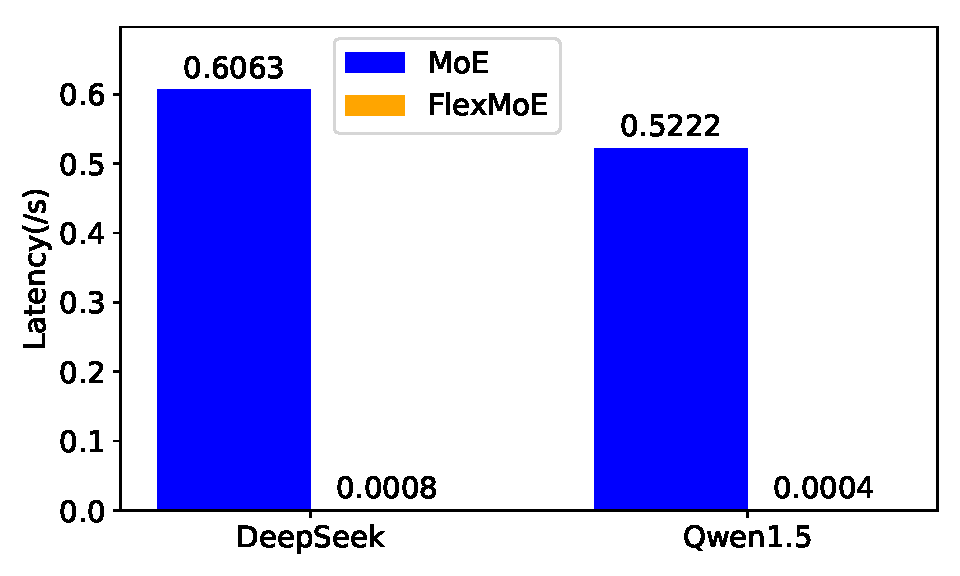
\includegraphics[width=0.99\linewidth]{figures/E2_910B.pdf}
        \caption{Ascend 910B}
    \end{subfigure}
    \caption{Overall waiting + cache-miss latency under memory-capped MoE inference (prompt length 8--1024).}
    \label{fig:E2}
\end{figure*}

We construct a test suite with prompt lengths from 8 to 1024 and
evaluate DeepSeek, Qwen1.5, and Qwen2.0 (where supported).
\autoref{fig:E2} shows that \systemname\ reduces the combined
waiting and cache-miss components relative to the baseline on every
device--model pair. The improvement is consistent across the three
heterogeneous platforms, indicating that \systemname\ adapts to
device-specific overlap opportunities rather than relying on a
single offline-tuned step size. The magnitude of reduction is
largest where expert transfer is on the critical path (Qwen1.5
exhibits the largest gains), and smaller but still positive where
the model already alleviates cache pressure architecturally (Qwen2.0,
whose shared experts~\cite{yang2024qwen2} partially absorb the
problem). Both latency components shrink together, which means
\systemname\ improves overlap without inducing cache thrashing.

A counter-intuitive cross-device data point reinforces the
runtime-control argument. H20's higher peak compute does not always
translate into lower end-to-end latency under our 20\,GB cap: at
small initial~$S$, H20 finishes per-layer compute quickly and then
stalls on transfers because effective bandwidth (and memory-allocator
overhead) does not scale with FLOPs. A6000's slower compute hides a
larger fraction of the same transfer naturally. This is exactly the
brittleness our motivation predicts---the optimal~$S$ shifts with
the compute-to-bandwidth ratio---and \systemname\ converges to
different~$S_t$ on the two devices, recovering the device-specific
overlap opportunity in both.

\subsection{Q2: Pre-Gate-Based Predictor}
\label{sec:eval:predictor}

We next isolate the contribution of the forecaster, since prediction
quality directly affects how often experts are resident when needed
and how much over-prefetch pollutes HBM. The forecaster operates on
token-level features and activation history, so its accuracy is
independent of GPU device; we therefore report it on A6000 as a
representative platform, evaluating 410 requests of varying lengths
under different step numbers when skipping layers in DeepSeek,
Qwen1.5, and Qwen2.0.

\begin{figure}
    \centering
    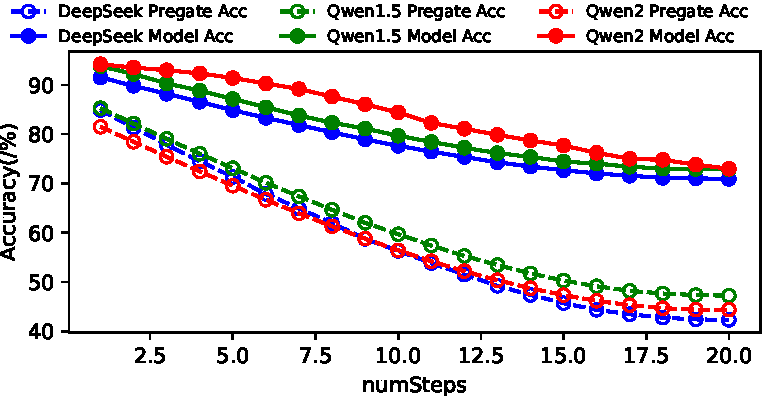
\includegraphics[width=0.99\linewidth]{figures/E1_pregate_model_with_markers.pdf}
    \captionsetup{belowskip=0em,aboveskip=0.0em}
    \vspace{-1.0em}
    \caption{Expert activation prediction accuracy: pregate vs.\ Predictor.}
    \label{fig:predictor-accuracy}
\end{figure}

\autoref{fig:predictor-accuracy} shows that the forecaster improves
accuracy consistently across all three model groups: the average gain
over pregate is $21.79\%$ (up to $30.36\%$). It also degrades more
smoothly as the prediction horizon grows, indicating better robustness
to long-range forecasting than pregate-only signals; compared with
ProMoE-style proactive prediction~\cite{song2024promoe}, the
forecaster achieves higher accuracy at the same step size.

Fitting both accuracy curves to an exponential decay, the asymptotic
accuracy gap $\Delta_\infty$ ranges from 30.8 to 37.0 percentage
points across the three model groups, confirming that the forecaster's
advantage over pregate-only signals is stable at long horizons.

\begin{figure*}[t]
    \centering
    \begin{subfigure}{0.32\linewidth}
        \centering
        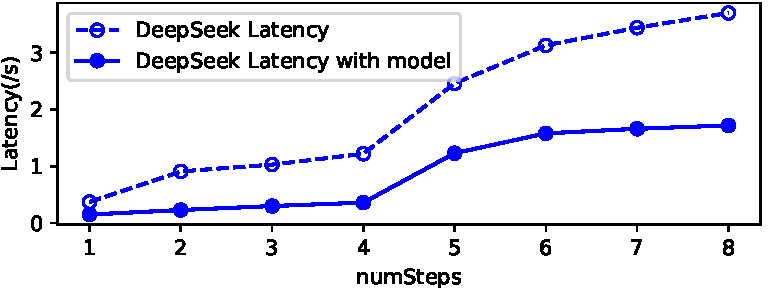
\includegraphics[width=0.99\linewidth]{figures/E1_Group1_Latency.pdf}
        \caption{DeepSeek-V2-Lite}
    \end{subfigure}
    \begin{subfigure}{0.32\linewidth}
        \centering
        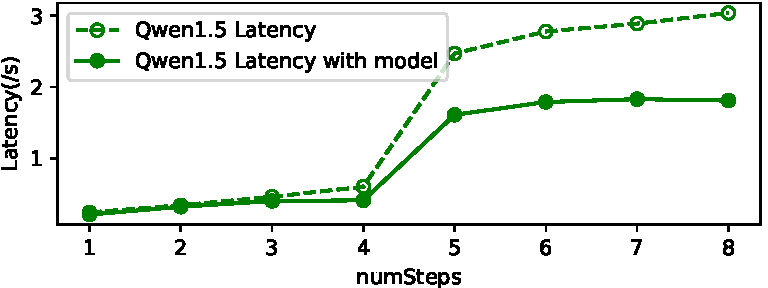
\includegraphics[width=0.99\linewidth]{figures/E1_Group2_Latency.pdf}
        \caption{Qwen1.5-MoE}
    \end{subfigure}
    \begin{subfigure}{0.32\linewidth}
        \centering
        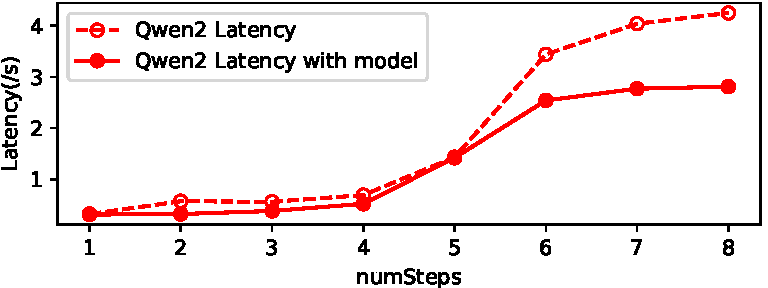
\includegraphics[width=0.99\linewidth]{figures/E1_Group3_Latency.pdf}
        \caption{Qwen2-MoE}
    \end{subfigure}
    \caption{Cache-miss latency after enabling the pregate-based Predictor.}
    \label{fig:E1_latency}
\end{figure*}

Under cross-layer prefetching, prediction errors incur two
complementary costs: under-forecasting misses required experts and
exposes waiting, while over-forecasting loads unused experts,
consuming bandwidth and polluting HBM. Improving prediction accuracy
therefore reduces both components, and \autoref{fig:E1_latency}
confirms this by showing that enabling the forecaster lowers
cache-miss latency across all model groups.

Tables~\ref{tab:Dynamic_baseline}--\ref{tab:Dynamic_predictor}
summarize the cache-miss latency component (seconds per request,
averaged over the 410-request suite at the representative
prompt-length bucket) under the baseline and the forecaster-enabled
configuration; ``--'' denotes a configuration that is unsupported
by the device's software stack under our 20\,GB cap. Values are
means over three runs (per-cell standard deviation $\le 6\%$ of the
mean). The forecaster gives an order-of-magnitude or larger
reduction on every supported configuration except Qwen2-MoE on H20,
where the baseline already overlaps most transfers; the latency
reduction there is correspondingly small but never negative. The
forecaster's robustness to long horizons is what lets the controller
push~$S$ higher when bandwidth is the bottleneck without paying a
misprediction tax.

\begin{table}[t]
\centering
\renewcommand{\arraystretch}{1.2}
\caption{Cache-miss latency (s/request) under the fixed-horizon baseline.}
\label{tab:Dynamic_baseline}
\resizebox{0.9\linewidth}{!}{
\begin{tabular}{c   c   c   c}
\hline\hline
\textbf{Model} & \textbf{A6000} & \textbf{H20} & \textbf{Ascend 910B} \\
\hline
DeepSeek-V2-Lite  & 1.38 & 0.46 & 0.61 \\
Qwen1.5-MoE       & 1.05 & 0.39 & 0.52 \\
Qwen2-MoE         & 1.77 & 1.16 & --   \\ \hline\hline
\end{tabular}
}
\end{table}

\begin{table}[t]
\centering
\renewcommand{\arraystretch}{1.2}
\caption{Cache-miss latency (s/request) with the Predictor enabled.
Reductions are largest where expert transfer dominates the critical
path; on configurations where the baseline already overlaps most
transfers (e.g., Qwen2-MoE on H20) the headroom is smaller, as expected.}
\label{tab:Dynamic_predictor}
\resizebox{0.9\linewidth}{!}{
\begin{tabular}{c   c   c   c}
\hline\hline
\textbf{Model} & \textbf{A6000} & \textbf{H20} & \textbf{Ascend 910B} \\
\hline
DeepSeek-V2-Lite  & 0.044 & 0.001 & 0.062 \\
Qwen1.5-MoE       & 0.038 & 0.038 & 0.069 \\
Qwen2-MoE         & 0.125 & 1.018 & --    \\ \hline\hline
\end{tabular}
}
\end{table}

\subsection{Q2: Memory Management Policy}
\label{sec:eval:memory}

We evaluate the contribution of our memory management policy, which provides
fine-grained control over expert swap operations via an LRU-style residency policy.
The key objective is to prevent pathological eviction--reload cycles that amplify
latency under limited GPU memory.

\begin{figure*}[t]
    \centering
    \begin{subfigure}{0.32\linewidth}
        \centering
        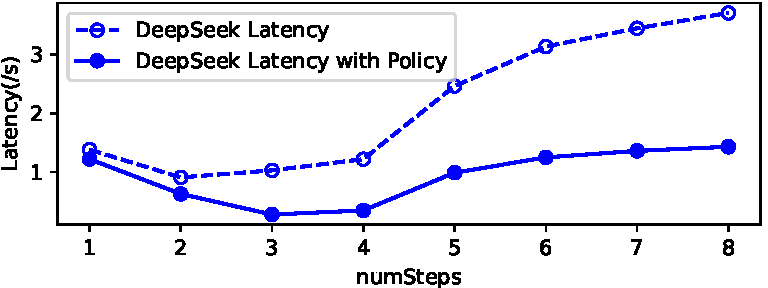
\includegraphics[width=0.99\linewidth]{figures/E3_Group1_Latency.pdf}
        \caption{DeepSeek-V2-Lite}
    \end{subfigure}
    \begin{subfigure}{0.32\linewidth}
        \centering
        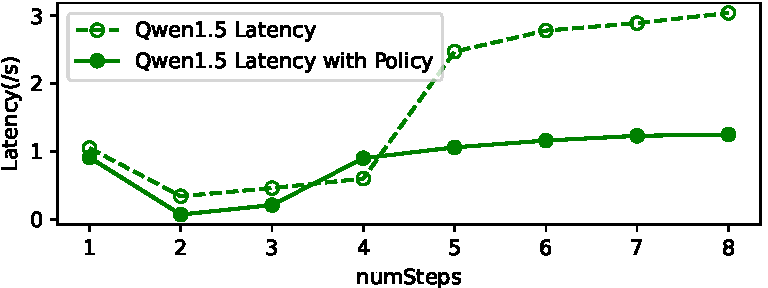
\includegraphics[width=0.99\linewidth]{figures/E3_Group2_Latency.pdf}
        \caption{Qwen1.5-MoE}
    \end{subfigure}
    \begin{subfigure}{0.32\linewidth}
        \centering
        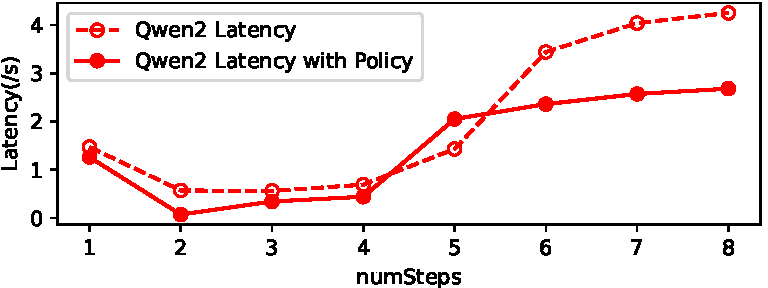
\includegraphics[width=0.99\linewidth]{figures/E3_Group3_Latency.pdf}
        \caption{Qwen2-MoE}
    \end{subfigure}
    \caption{Latency under cross-layer prediction with the proposed memory management policy.}
    \label{fig:E3_latency}
\end{figure*}

\autoref{fig:E3_latency} shows that enabling the two-tier policy
consistently reduces latency compared to the baseline without
dedicated swap-out control. Even with the same forecasting
mechanism, controlling which experts remain resident in HBM is
essential for stabilizing performance under tight memory budgets.
The most informative point is the latency spike that the baseline
exhibits near $S \approx 4$: larger step sizes increase prefetch
depth and short-term residency demand, and once this demand exceeds
the memory cap, eviction--reload cycles amplify latency. The
two-tier residency policy flattens this cliff into a plateau by
localizing the cost of misprediction to a single DMA rather than
triggering an eviction--reload cascade. This is what
makes the controller's exploration of larger~$S$ safe.

\subsection{Q3: Cache-aware Routing}
\label{sec:eval:routing}

Finally, we evaluate cache-aware routing, which couples routing decisions with
current cache residency to reduce cache misses and transfer-induced stalls.
This mechanism is designed to complement both the Predictor and the memory
management policy by reducing the probability that routing selects experts that
are expensive to materialize under current memory pressure.

\begin{figure*}[htp]
    \centering
    \begin{subfigure}{0.32\linewidth}
        \centering
        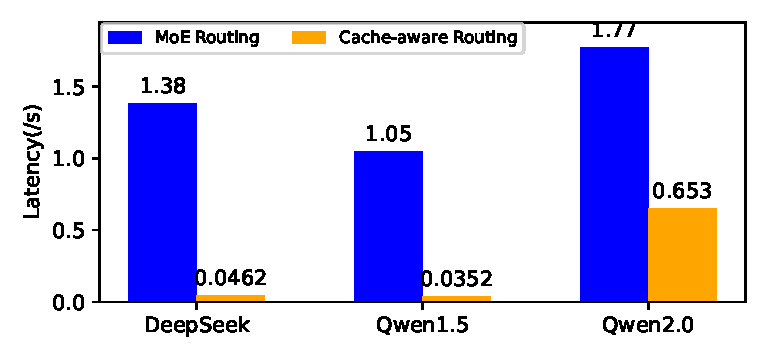
\includegraphics[width=0.99\linewidth]{figures/E4.pdf}
        \caption{NVIDIA A6000}
    \end{subfigure}
    \begin{subfigure}{0.32\linewidth}
        \centering
        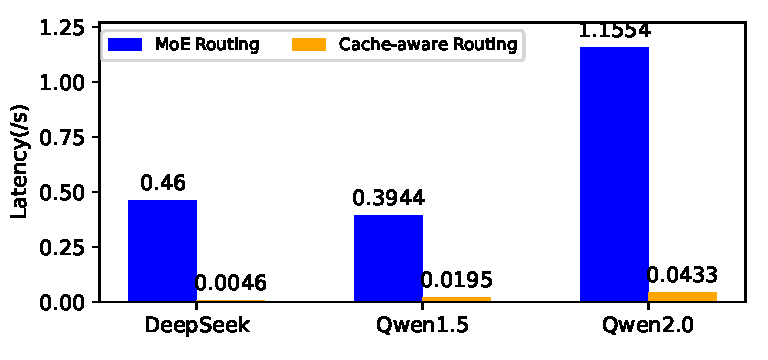
\includegraphics[width=0.99\linewidth]{figures/E4_H20.pdf}
        \caption{NVIDIA H20}
    \end{subfigure}
    \begin{subfigure}{0.32\linewidth}
        \centering
        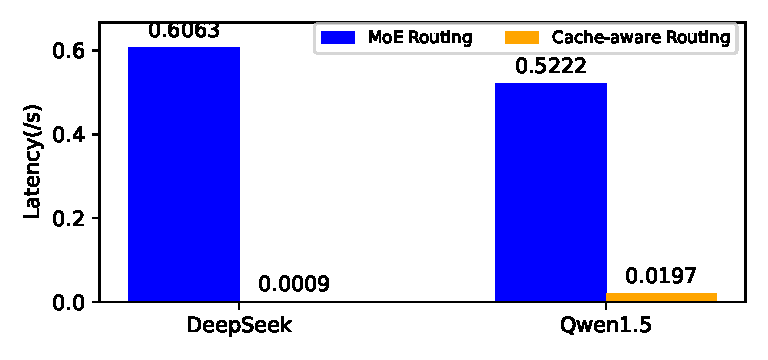
\includegraphics[width=0.99\linewidth]{figures/E4_910B.pdf}
        \caption{Ascend 910B}
    \end{subfigure}
    \caption{End-to-end latency comparison with and without cache-aware routing.}
    \label{fig:cache-aware-routing}
\end{figure*}

\autoref{fig:cache-aware-routing} shows that cache-aware routing
reduces end-to-end latency across DeepSeek, Qwen1.5, and Qwen2.0 by
mitigating expert-loading delays and cache misses. The relative
improvement is strongest for DeepSeek and Qwen1.5, which are more
sensitive to swapping-induced instability under our memory cap.
Qwen2.0 benefits as well, although its built-in shared-expert
design~\cite{yang2024qwen2} already alleviates some cache
inefficiencies; cache-aware routing is therefore complementary
rather than redundant.
\autoref{tab:Dynamic_CCR} reports the cache-miss latency component
(s/request, mean of three runs; same methodology as
Tables~\ref{tab:Dynamic_baseline}--\ref{tab:Dynamic_predictor}) with
cache-aware routing further enabled on top of the forecaster and
the two-tier cache. The largest reduction is on H20, consistent
with its higher compute throughput exposing relatively more transfer
time when routing is cache-oblivious. Combined with the controller
and forecaster, the routing layer closes the loop: prediction errors
that survive the cache no longer propagate into stalls.

\begin{table}[t]
\centering
\renewcommand{\arraystretch}{1.2}
\caption{Cache-miss latency (s/request) with cache-aware routing enabled.}
\label{tab:Dynamic_CCR}
\resizebox{0.9\linewidth}{!}{
\begin{tabular}{c   c   c   c}
\hline\hline
\textbf{Model} & \textbf{A6000} & \textbf{H20} & \textbf{Ascend 910B} \\
\hline
DeepSeek-V2-Lite  & 0.033 & 0.003 & 0.002 \\
Qwen1.5-MoE       & 0.022 & 0.002 & 0.002 \\
Qwen2-MoE         & 0.103 & 0.098 & --    \\ \hline\hline
\end{tabular}
}
\end{table}

\subsection{Runtime Overhead}
\label{sec:eval:overhead}

We separately measure the overhead of the three layers introduced by
\systemname\ to confirm that they do not displace the gains shown in
Q1--Q3. The controller's per-update cost is bounded by \autoref{alg:controller}
to a few EMA updates and a comparison; we measure it at $<50\,\mu$s
on a commodity CPU across all evaluated workloads, which is at least
two orders of magnitude smaller than per-layer compute on every
device. The forecaster runs on the same CPU thread as the
controller; its prediction at control-period granularity is
sub-millisecond and never appears on the GPU critical path, so its
amortized cost is dominated by the per-epoch retraining that runs
between requests. The memory layer's two-tier LRU operates on block
indices and a single asynchronous DMA per eviction, with the
allocator-side cost hidden by the dedicated transfer stream and not
visible in the latency components reported above. Aggregated across
the three layers, the wall-clock overhead introduced by \systemname\
is below the noise floor of our latency-attribution instrumentation,
so the cache-miss reductions in
Tables~\ref{tab:Dynamic_baseline}--\ref{tab:Dynamic_CCR} are net of
all framework costs.


\section{Discussion and Limitations}
\label{sec:discussion}

\textbf{Workload regimes with limited gains.}
\systemname\ targets the regime in which expert transfer is on (or
near) the critical path. When effective transfer bandwidth is high
enough that the baseline already overlaps most transfers (e.g.,
Qwen2-MoE on H20 in \autoref{sec:evaluation}), the controller
converges to a small~$S$ and contributes only the
$O(L_{\text{MoE}})$ controller overhead, which we measure to be
under $50\,\mu$s per update on a commodity CPU. We did not observe a
configuration in which \systemname\ degraded the baseline, but we do
not claim universal speedups: a model whose entire expert footprint
fits in HBM under the deployment cap, or a workload whose routing is
so concentrated that one or two experts cover it, gains little from
adaptive prefetching.

\textbf{Memory-cap sensitivity.}
Our evaluation fixes a 20\,GB HBM cap to expose expert-residency
contention on every device under study. The cap was chosen to
emulate consumer GPUs and multi-tenant deployments where KV-cache,
activations, and other tenants compete for HBM with expert weights;
it does not represent the only operating point of interest. The
behavior of \systemname\ at smaller caps (10\,GB) is bounded by the
$S_{\min}$ floor of the controller, which prevents thrashing at the
cost of losing some overlap; at larger caps the controller converges
to higher~$S$ and gains diminish as more experts become persistently
resident. Characterizing this curve quantitatively is left to future
work; we expect the qualitative trend to mirror
\autoref{fig:M1}, since the underlying overlap--pollution tradeoff
is the same.

\textbf{Multi-stream and multi-tenant deployment.}
\systemname\ targets a single-stream serving setup with continuous
batching. Co-locating multiple model instances on a single GPU
introduces inter-instance contention on the transfer stream and on
HBM, which the current controller does not explicitly model: each
instance optimizes its own~$S$, and contention manifests in the
shared bandwidth estimate~$C_s$. We expect the per-instance
controller to remain stable (because (C2) bounds per-step change to
$\pm1$), but the joint optimum may not match the union of local
optima. Lifting the controller to a coordinated multi-stream
setting---potentially by sharing $C_s$ and $\tilde{m}_t$ across
instances---is a natural extension.

\textbf{Predictor cold start and online retraining.}
The forecasting layer relies on a CPU-side random forest trained
offline from logged tuples. On a previously unseen model or
substantially shifted workload, the forecaster falls back to the
model's own pregate top-$k$, which we measured matches the
fixed-horizon baseline. The system therefore degrades gracefully
rather than catastrophically. Online retraining (incremental forest
updates as new $(\mathbf{t},\ell,S,\mathbf{a})$ tuples arrive) is
straightforward to add and does not interact with the controller's
stability proof, but we have not characterized its convergence
empirically.

\textbf{Threats to generality.}
Our experiments cover three MoE models from the DeepSeek and Qwen
families and three accelerators spanning a $4\times$ effective-bandwidth
range. We did not evaluate Mixtral-class models (which use a different
expert sizing) or larger DeepSeek-V3-class models; we expect the same
mechanism to apply, but the optimal hyperparameters
($\lambda, \theta_h$) may shift. We also do not evaluate disaggregated
or pipeline-parallel deployments, where prefetch coordination crosses
device boundaries.
\section{Related Work}
\label{sec:related_work}

\subsection{MoE Inference Systems}
Early sparse-activation designs such as the Switch Transformer~\cite{fedus2021switch} demonstrated that routing each token to a small subset of experts substantially reduces computation while preserving model capacity. Subsequent serving systems strengthened this direction by addressing communication and scheduling costs at large scale~\cite{riquelme2021scaling, li2025uni, zhu2025exploring, zhang2025duoservemoe, yu2025prescope}. ExFlow~\cite{yao2024exploiting} leverages inter-layer expert affinity to colocate frequently co-activated experts, while TA-MoE~\cite{chen2022ta} uses device topology to reduce cross-node transfers. These approaches reduce communication but assume that expert availability can be largely predicted offline.

A separate line of work targets memory pressure on commodity or memory-constrained GPUs. ProMoE~\cite{song2024promoe}, ExpertFlow~\cite{he2024expertflow}, and Hobbit~\cite{tang2024hobbit} all employ cross-layer prefetching with a fixed forecasting horizon. ExpertFlow integrates token-aware expert prediction with proactive caching; Hobbit relies on mixed-precision offloading and multi-level caches; MoE-Lightning~\cite{cao2024moe} introduces hierarchical memory management to rebalance expert residency mid-execution. Other systems prioritize experts already in fast memory~\cite{bambhaniya2024moe} or inject null experts to smooth routing dynamics~\cite{zeng2024adamoe}. \systemname\ differs from all of the above by treating the prefetch horizon as a runtime control variable rather than an offline-tuned hyperparameter, by closing a feedback loop between stall/eviction signals and the horizon decision, and by letting cache-aware token routing absorb residual misprediction inside resident-expert compute.

\subsection{Routing and Load Balancing}
Routing quality is a central determinant of MoE efficiency~\cite{huang2025dynamic, zhou2025moe}. Expert Choice~\cite{zhou2022mixture} provides load balancing by letting experts self-select tokens; AdaMOE~\cite{zeng2024adamoe} dynamically adjusts the number of active experts per token; ExFlow~\cite{he2024expertflow} maintains routing consistency across layers to reduce communication; MoDSE~\cite{sun2024mixture} assigns heterogeneous expert sizes to match input complexity. These techniques shape \emph{which} experts are activated. \systemname\ is orthogonal: rather than designing new routing objectives or expert topologies, we treat the cross-layer prediction interval as a runtime control variable, leaving routing semantics unchanged. The two directions are complementary, and \systemname\ can be deployed in front of any of the routing schemes above.

\section{Conclusion}
\label{sec:conclusion}

In this paper we present \systemname, a serving runtime designed for
memory-constrained Mixture-of-Experts inference under
expert-residency contention.
\systemname\ realizes the idea of treating the cross-layer prefetch
horizon~$S$ as a \emph{runtime control variable}: a bounded $\pm 1$
update with hysteresis on EMA-smoothed stall and eviction signals
picks a different~$S_t$ at each control period.
This reframing breaks the brittle dependence of fixed-horizon
prefetching on hardware and workload, recovering the per-configuration
optimum that no single offline~$S$ can match.
A CPU-side delta-adjusted forecaster and a residency-aware two-tier
expert cache with cache-aware token routing make this control loop
safe by bounding the cost of every prediction error to a single DMA.
Our evaluation across three accelerators and three MoE models
demonstrates that \systemname\ reduces cache-miss latency by an
order of magnitude on most configurations while never degrading the
ones where the baseline is already near-optimal.

%-------------------------------------------------------------------------------
% Acknowledgments are omitted for double-anonymous review (per ICPP 2026 CFP).
% \section*{Acknowledgements}
\label{sec:acknowledge}
This document is derived from previous conferences, in particular ISCA 2019, MICRO 2019, ISCA 2020, MICRO 2020, ISCA 2021, HPCA 2022, ISCA 2022, ISCA 2023, and ISCA 2024. We thank the organizers of MICRO 2022 for the idea to set up HotCRP topic selections.
%-------------------------------------------------------------------------------

\bibliographystyle{ACM-Reference-Format}
\bibliography{references}

%%%%%%%%%%%%%%%%%%%%%%%%%%%%%%%%%%%%%%%%%%%%%%%%%%%%%%%%%%%%%%%%%%%%%%%%%%%%%%%%
\end{document}
%%%%%%%%%%%%%%%%%%%%%%%%%%%%%%%%%%%%%%%%%%%%%%%%%%%%%%%%%%%%%%%%%%%%%%%%%%%%%%%%
